\documentclass[a4paper,12pt]{article}

\usepackage{fontspec}
\usepackage{amsmath}
\usepackage{enumitem}
\usepackage[subrefformat=parens,labelformat=parens]{subfig}
\usepackage[a4paper,margin=1in]{geometry}

\newcommand{\eqname}[1]{\tag*{#1}} % tag an equation with a name

\defaultfontfeatures{Mapping=tex-text}
\setromanfont[Ligatures={Common},Numbers={Lining}]{Linux Libertine}

\title{Applied Estimation Lab 1---Extended Kalman Filter}
\author{Michal Staniaszek}

\begin{document}
\maketitle

\section{Part I---Preparatory Questions}
\subsection{Kalman Filter}
\begin{enumerate}
\item A control is something that is applied to the system to modify its
  state. The control can be controlled by us, or it can be another process which
  we model, but have no control over. A measurement is information that we
  receive about the state of the environment based on some sensor reading, or
  other measuring device, which does not necessarily give direct information
  about the state of the system. The state is a set of parameters which
  represent the system that we are working with. The state is what we are trying
  to estimate the evolution of, given the controls and measurements received.
\item It is not possible for the uncertainty to increase during an update. It
  naturally increases when a control is applied due to the uncertainty of the
  state transition, but since information is \emph{gained} when we receive a
  measurement, the uncertainty will always decrease. This can be verified by
  looking at the covariance matrix update equation:
  \begin{align*}
    \Sigma_t=(I-K_tC_t)\bar{\Sigma}_t
  \end{align*}
  We know that the product $K_tC_t$ will produce a matrix which is positive
  semidefinite, and therefore subtracting this from the identity will result in
  the multiplication of $\bar{\Sigma}_t$ by a fractional value. Thus, $\Sigma_t$
  will have smaller values in it than $\bar{\Sigma}_t$. The smaller the values
  in $\Sigma_t$, the tighter the Gaussians, and the lower the uncertainty. It
  should be noted that the estimate is different from the true state. Even if
  the uncertainty in the estimate goes down, the error between the true
  state and the estimated state can increase due to a sub-optimal model.
\item The weighting between measurements and belief is the Kalman gain
  $K_t$. The gain is computed and used in the update step to modify both the new
  mean $\mu_t$ and covariance matrix $\Sigma_t$. The measurement update is done
  using
  \begin{align*}
    \mu_t=\bar{\mu}_t+K_t(z_t-C_t\bar{\mu}_t)
  \end{align*}
  The part of the measurement $z_t$ added to $\mu_t$ is proportional to $K_t$,
  and therefore $K_t$ defines how much it is taken into consideration. The size
  of $K_t$ is influenced by $\bar{\Sigma}$ and $Q_t$, the predicted covariance
  and measurement noise respectively, which means that the size of the
  uncertainty, and the unreliability of measurements affect the gain.
\item The effect of changes in $Q_t$, the measurement noise, can be investigated
  by looking at the computation of $K_t$:
  \begin{align*}
    K_t=\bar{\Sigma}_tC^T_t(C_t\bar{\Sigma}_tC^T_t+Q_t)^{-1}
  \end{align*}
It is easier to see the effects of a large $Q_t$ in the scalar case:
\begin{align*}
  k_t&=c_t\bar{\sigma}_t(c^2_t\bar{\sigma}_t+q_t)^{-1}\\
  &=\frac{c_t\bar{\sigma}_t}{c^2_t\bar{\sigma}_t+q_t}
\end{align*}
As $q_t$ tends to infinity, we get
\begin{align*}
  k_t=\lim_{q_t\to \infty}\frac{c_t\bar{\sigma}_t}{c^2_t\bar{\sigma}_t+q_t} \approx 0
\end{align*}
So, as $q_t$ increases, the Kalman gain tends towards zero, meaning that
measurements will not be considered at all in the update step. This is also the
case in the non-scalar case.
\item For the measurements to have an increased effect, the Kalman gain must
  increase. As seen above, as $q_t\to \infty$, $k_t\to 0$. It is easy to see
  that as $q_t \to 0$, $k_t\to \frac{1}{c_t}$. This indicates that reducing the
  uncertainty $Q_t$ in the measurements will increase the gain. In addition,
  the value of $c_t$ (or structure of $C_t$) may also have some effect on the
  gain.
\item During prediction, the belief uncertainty increases. Intuitively, this
  happens because we are uncertain about the state transitions that are being
  made, depending on the uncertainty $\epsilon_t$, modeled by $R_t$. Because we
  could transition to any number of states after making a transition, there is
  no way that we could \emph{decrease} the uncertainty.
  
  \begin{align*}
    \bar{\Sigma}_t=A_t\Sigma_{t-1}A^T_t+R_t
  \end{align*}

  Since $\Sigma_{t-1}$ is positive semidefinite, multiplying it by $A_t$, which
  has the same property, results in larger values in the matrix. Adding the
  measurement covariance $R_t$ further increases this uncertainty.
\item If the true distributions of the measurement and state transition noise
  are indeed Gaussians as we have assumed, then it follows that there can be no
  distribution that better estimates the true distribution. It can be shown that
  if instead of using the means predicted by the Gaussians we use a different
  mean, then a worse estimate results.
\item In a MLE, we assume that nothing is known about the distribution of the
  initial state, which means that the distribution is uniform. In a MAP, a prior
  is used in the computation of the posterior. Generally, when using a Kalman
  filter, we do not know anything about the initial distribution, and so ideally
  we would use a uniform distribution. However, since the KF uses Gaussian
  representations, we cannot do this. As a result, the KF is really a MAP
  estimator, but in some sense it could be said to be both.
\end{enumerate}
\subsection{Extended Kalman Filter}
\begin{enumerate}[resume]
\item The extended Kalman filter is an extension of the Kalman filter to systems
  with non-linear state transitions. This extension destroys some of the good
  properties of the Kalman filter, but is used much more in practice because
  most systems are non-linear in some way. In the EKF, the state transition
  matrix $A_t$ is replaced with a Jacobian $G_t$ based on the linearisation of
  the state transition function $g(u_t,\mu_{t-1})$, which approximates the
  effect of noise on the non-linear state transition as a linear function. The
  measurement equation is also modified to use a Jacobian $H_t$ instead of
  $C_t$, again representing the linearised measurement function.
\item The EKF is not guaranteed to converge. Divergence can be caused by various
  factors, such as an incorrect model, measurement correlations or bias,
  disturbances, or problems with the matrix structures. The convergence also
  depends on the linearisation. If the state transition function is highly
  nonlinear, then the linearisation may be inaccurate when the uncertainty is
  large due to variation in the nonlinear function.
\item To reduce the divergences, we can increase the uncertainty parameters that
  are being used. This means that the filter will be less certain about the
  evolution of the system, and less likely to diverge because of an estimate
  that has relatively low uncertainty, but is in fact incorrect. If the
  divergence is due to bad data association, then we can change the matching
  threshold that is being used.
\end{enumerate}
\subsection{Localisation}
\begin{enumerate}[resume]
\item If the robot is completely unsure of its location, then the prior is a
  Gaussian with a high covariance. After seeing the landmark, all that can be
  deduced is that the robot must be somewhere on the circumference of the circle
  of radius $r$ centred on the landmark, with the added Gaussian noise creating
  a ring, with probabilities decreasing towards the edges of the ring. Because
  it is not possible to represent this ring shape with a Gaussian, the estimate
  will likely place the mean on top of the landmark, with a large covariance to
  cover the whole ring. A single landmark is not enough to actually localise,
  since it does not give enough information.
\item If the measurement also includes a bearing, we can deduce that the robot
  must be facing in a specific direction, but we do not gain any additional
  information about its position, as that is determined by the range measurement
  alone in the situation with which we are presented. The distribution of
  possible positions is still a ring, but we now know that the orientation of
  the robot is dependent on its position on the ring.
\item Since we have good motion estimation, we know approximately how far we
  will move in the direction of motion. However, because the initial bearing is
  uncertain, the uncertainty on the Gaussian perpendicular to the direction of
  motion would be large, indicating that in actual fact the position could be
  quite far from the mean in that direction. The ideal distribution would be
  banana shaped (depending on the initial uncertainty), but since we must
  represent it as a Gaussian, it must be approximated as best as possible. The
  heading will be correlated with the position on the arc.
\item There are numerous reasons for why an EKF update could go wrong due to a
  measurement. The most obvious of these is a spurious sensor reading, which
  appears to detect a feature when it is not in fact there. Issues could also be
  caused by data processing errors which again result in the detection of a
  feature which does not exist. If such a measurement was received by the EKF,
  particularly one using a sequential update, then if it is taken into account
  then the update becomes inconsistent; something has been measured and taken
  into account, modifying the belief, when in fact it should have been
  discarded. Since the EKF uses Gaussians, if the landmark is not unique, we are
  not necessarily able to update the posterior to reflect the true state. All
  that we can say is that we are near some landmark, and we must compromise to
  choose only the one which has the maximum likelihood at the time. If we
  started off with very little information about bearing, then the landmark that
  we end up choosing as the one we thing we are close to could be the wrong one,
  and the posterior will be moved to an incorrect location. In general, because
  it is not possible to represent the posterior with a Gaussian, the
  linearisation is not accurate and this could lead to a bad update. 
\end{enumerate}
\section{Part II---Matlab Exercises}
\subsection{Kalman Filter}
\begin{enumerate}
\item The dimensions of $\epsilon_k$ correspond to the number of parameters
  required to represent the state~$x_t$. Each element of $\epsilon_k$ represents
  the noise inherent to that parameter of the state during the state
  transition. In the example of the car, $\epsilon_k$ is a $2\times 1$ vector,
  with noise for both position and velocity. $\delta_k$ is the noise that is
  present in the measurement. Its dimensions depend on the length of the
  measurement vector. If we consider each element of this vector to be a
  measurement from a different sensor, it is natural to have different noise for
  each. In the car example, $\delta_k$ is a scalar value, as there is only one
  thing that is being measured, the position of the car. In the scalar case, a
  Gaussian, or normal distribution is characterised by a mean~$\mu$ and a
  variance~$\sigma^2$ around that mean, and is generally represented by
  $\mathcal{N}(\mu,\sigma^2)$. In the vector case, $\mu$ becomes a vector, and
  $\sigma^2$ a matrix. The notation for $\mu$ is the same, but the variance is
  represented by the \emph{covariance matrix}~$\Sigma$, and as such a
  multivariate Gaussian is represented by $\mathcal{N}(\mu,\Sigma)$. A white
  Gaussian is one with zero mean and a diagonal covariance matrix, such that the
  noise in one parameter is not correlated with any other.
\item 
  \begin{description}
  \item[$x$] A $2\times 1$ vector representing the true state of the
    system. Contains the position and velocity of the car at each time step.
  \item[$\hat{x}$] A $2\times 1$ vector representing the state of the car
    estimated by the KF. Contains an estimate of the position and velocity of
    the car at each time step. This is the state vector that is used by the
    KF---we have no access to the true state.
  \item[$P$] A $2\times 2$ covariance matrix representing the uncertainty of the
    current EKF estimate. Contains either the predicted covariance
    $\bar{\Sigma}$ or the updated covariance $\Sigma$, depending on which point
    in the code execution is at. Used to compute both the Kalman gain $K$ and
    the covariance after prediction or update.
  \item[$G$] A multiplier on the noise model for the state transitions to get
    the correct matrix dimensionality.
  \item[$D$] A multiplier on the noise model for the measurements to get the
    correct matrix dimensionality.
  \item[$Q$] A $2\times 2$ matrix. The noise model for the state
    transition. This indicates the estimates that we have made of the true noise
    in the system for each parameter in the state. In the ideal case, this
    matrix contains the values of $wStdP^2$ and $wStdV^2$. If the noise is lower
    than the true noise, then the estimator will be optimistic, and if the noise
    is higher then it will be pessimistic. Both of these can cause problems,
    either with overconfidence in bad estimates, or too little confidence in
    quite a good estimate.
  \item[$R$] A scalar value. The noise model for the measurements. Indicates an
    estimate of the true noise on the measurements that we will receive from
    our simulated sensor. The ideal value for this is the actual noise on the
    measurements, which is represented by $vStd$.
  \item[$wStdP$] The true variance of the noise in the position. The noise is
    added to the system by generating a normally distributed random number with
    a zero mean and variance~$wStdP$.
  \item[$wStdV$] The true variance of the noise in the velocity. The noise is
    added to the system by generating a normally distributed random number with
    zero mean and variance~$wStdP$.
  \item[$vStd$] The true variance of the noise in the measurement. This is added
    to the measurement at each time step by generating a normally distributed
    random number with zero mean and variance of~$vStd$.
  \item[$u$] The control applied to the system at each time step, that is, the
    instantaneous acceleration of the car, which is assumed to be constant
    between time steps. Setting this to zero will mean that the system is driven
    by the noise $wStdP$.
  \item[$PP$] Stores the values of the covariance matrix after the update step
    at each time step such that they can be plotted later to examine the
    evolution of the covariance over time.
  \end{description}
\item In Figure~\subref*{fig:hiq}, we increase $Q$, giving a higher process
  noise estimate. From this we would expect that our measurements would be
  trusted more, as our motion is uncertain. This is confirmed by comparing the
  Kalman gain with Figure~\subref*{fig:def}. We see that the steady state gain
  for both range~$K1$, and speed~$K2$ is higher, so we give the measurements
  higher weight. As a result of the higher process noise, the tracking of the
  speed suffers, it is much more difficult to predict. With low process noise,
  we expect measurements to receive a lower weight, as our process is more
  predictable. This is clear from the low gain in both position and velocity in
  Figure~\subref*{fig:loq}. Additionally, we have a lower steady state
  covariance as we are more certain about how the system evolves. As a result of
  the low gain, tracking of the true state is smoother, and has a slight
  lag. $R$ represents the measurement noise model. A higher measurement noise
  means that we put less weight on our measurements as they are unreliable. High
  measurement noise keeps the gain low, and has a large effect on the
  convergence time of the system. Tracking of the true state is smooth, as the
  measurements do not force the estimate to move much
  (Figure~\subref{fig:hir}). With low measurement noise, the gain is high, and
  so measurements have a large effect on the system. This results in a rapidly
  changing estimate of both the position and the speed. When both $Q$
  and $R$ are high, we are uncertain about both the process and the
  measurements. As a result, the Kalman gain is low, and the steady state
  covariance is high. The result is slow convergence to the true state, as the
  update is more cautious about updates. With both low, we have more
  contribution from the measurements, and a very low steady state covariance. In
  both cases, the tracking of the speed does not undergo any significant change,
  which can be seen in Figure~\ref{fig:prop}.

  \begin{figure}
    \subfloat[High noise: $Q\times 100,R\times 100$]{
      \centerline
      {
        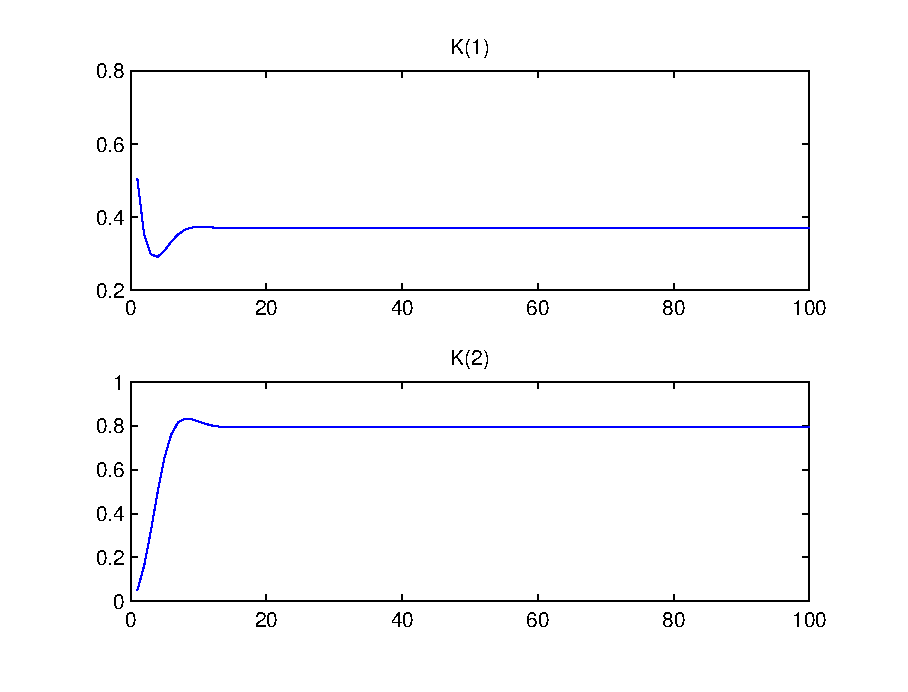
\includegraphics[width=.43\textwidth]{figures/kf/rqhigh_kalman}
        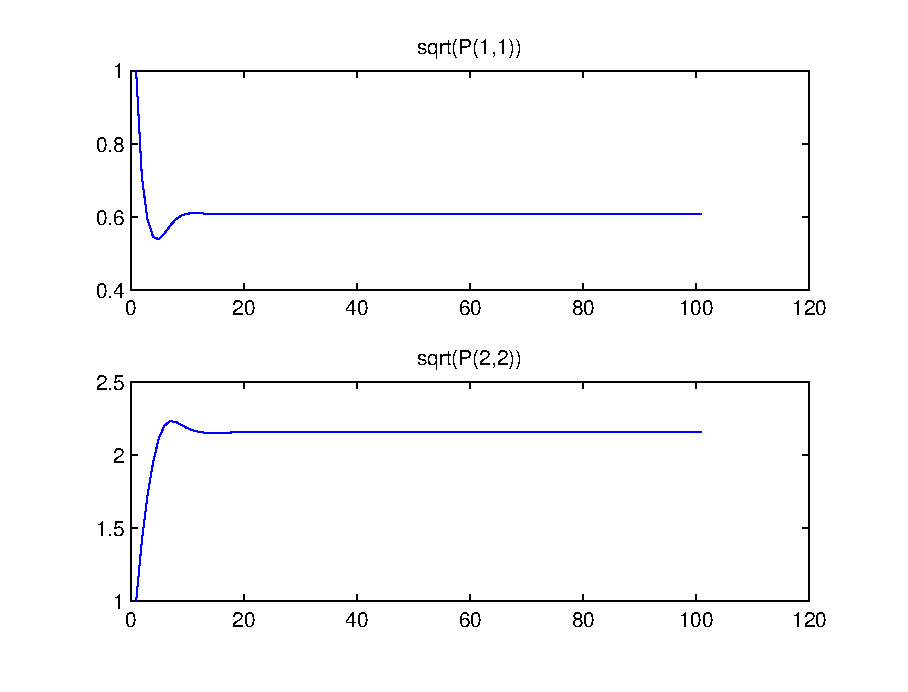
\includegraphics[width=.43\textwidth]{figures/kf/rqhigh_covar}
        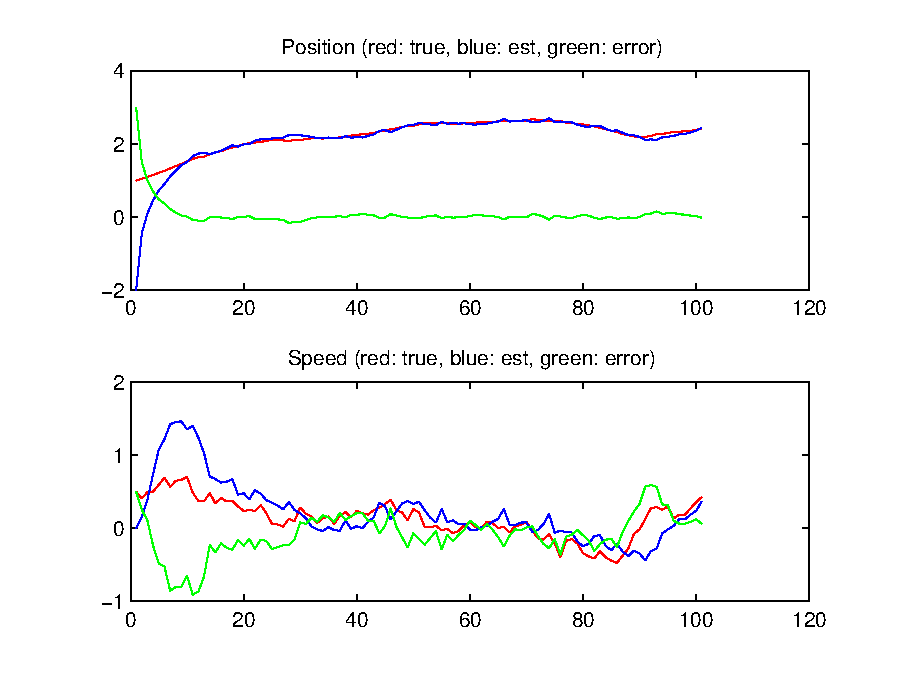
\includegraphics[width=.43\textwidth]{figures/kf/rqhigh_error}
      }
    }\\
    \subfloat[Low noise: $Q/100,R/100$]{
      \centerline
      {
        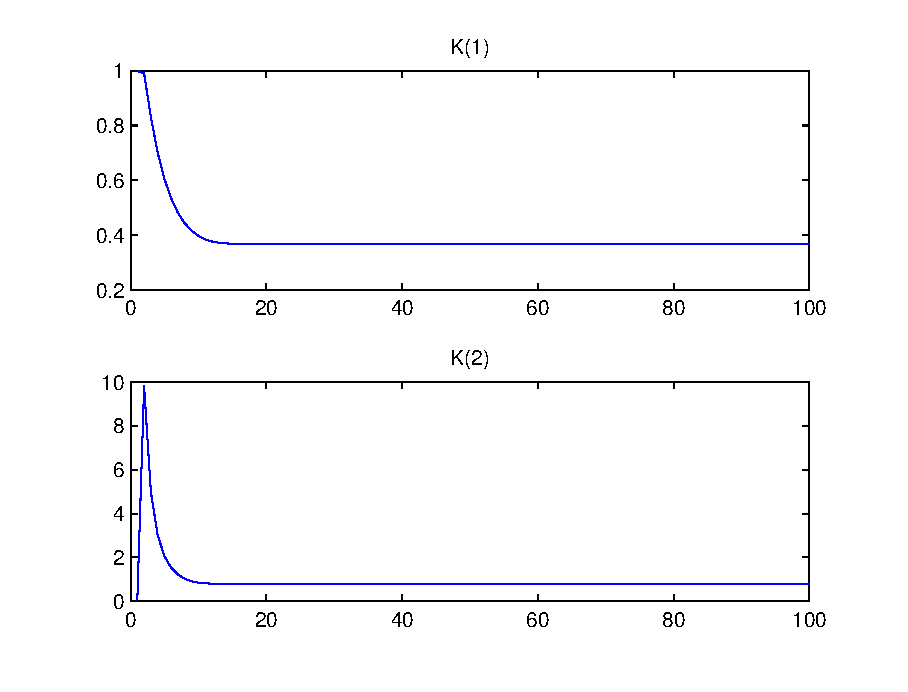
\includegraphics[width=.43\textwidth]{figures/kf/rqlow_kalman}
        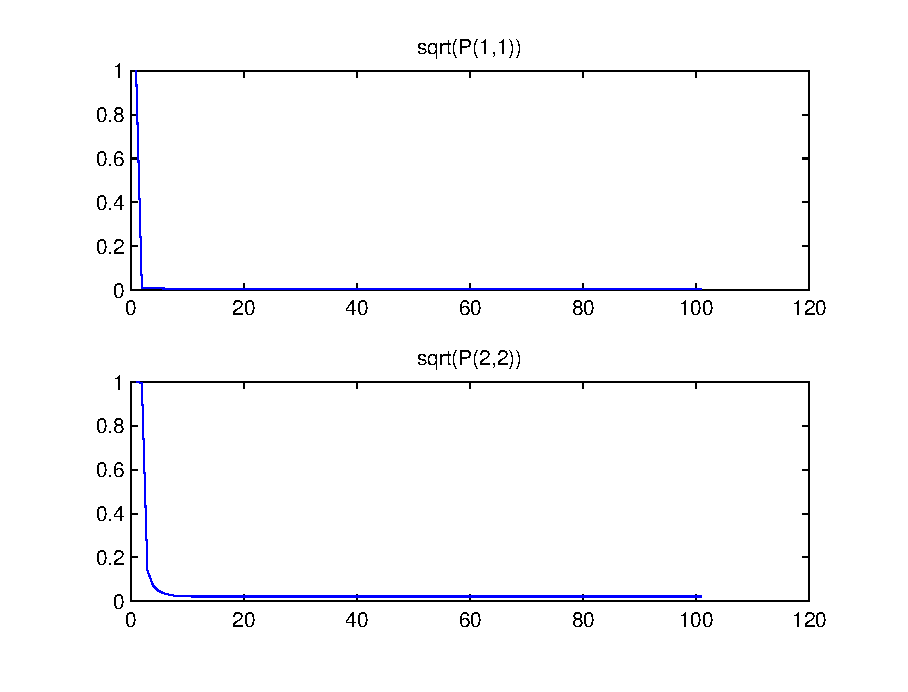
\includegraphics[width=.43\textwidth]{figures/kf/rqlow_covar}
        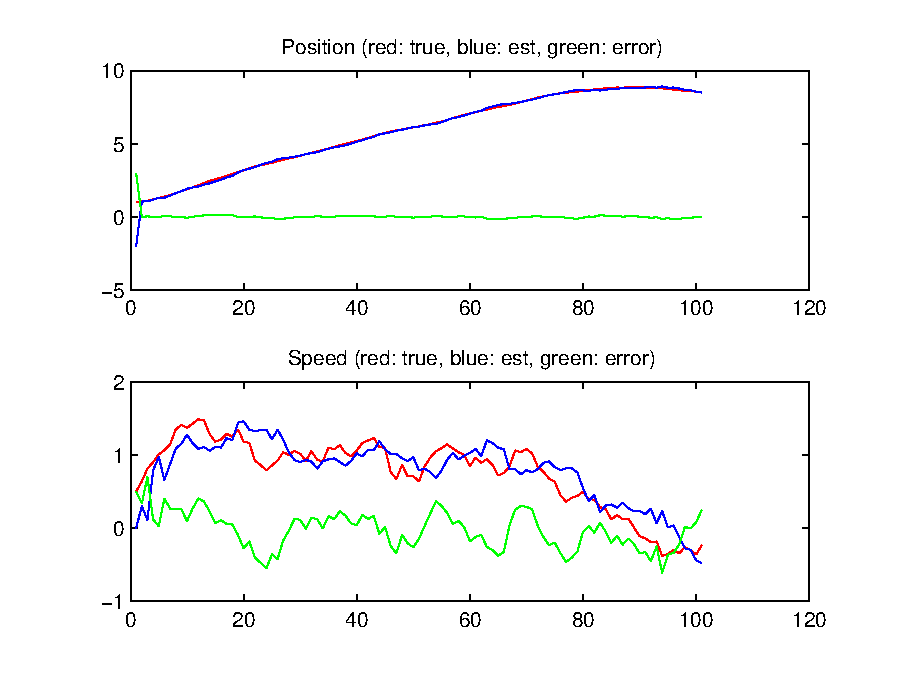
\includegraphics[width=.43\textwidth]{figures/kf/rqlow_error}
      }
    }
    \caption{Graphs for different process and measurement noise models, from
        left to right the Kalman gain, covariance and error. By default,
        $Q=$\texttt{diag}$(0.0001,0.01)$, $R=0.01$. Here, we change both $Q$ and
      $R$ by the same proportion.}
    \label{fig:prop}
  \end{figure}
  
  \begin{figure}
      \subfloat[Normal: $Q=$\texttt{diag}$(0.0001,0.01)$, $R=0.01$.]{
        \centerline
        {
          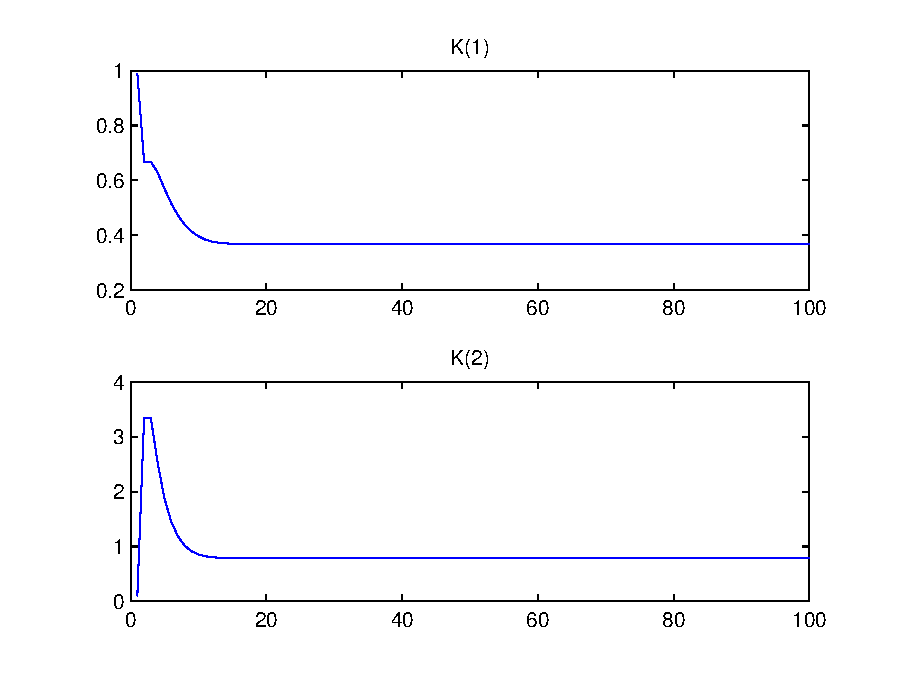
\includegraphics[width=.43\textwidth]{figures/kf/norm_kalman}
          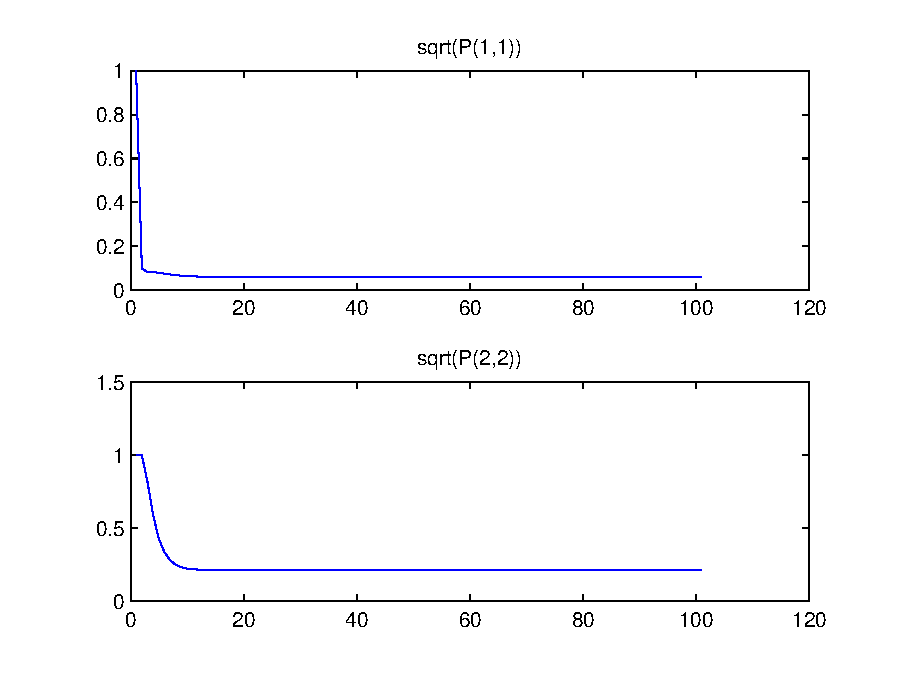
\includegraphics[width=.43\textwidth]{figures/kf/norm_covar}
          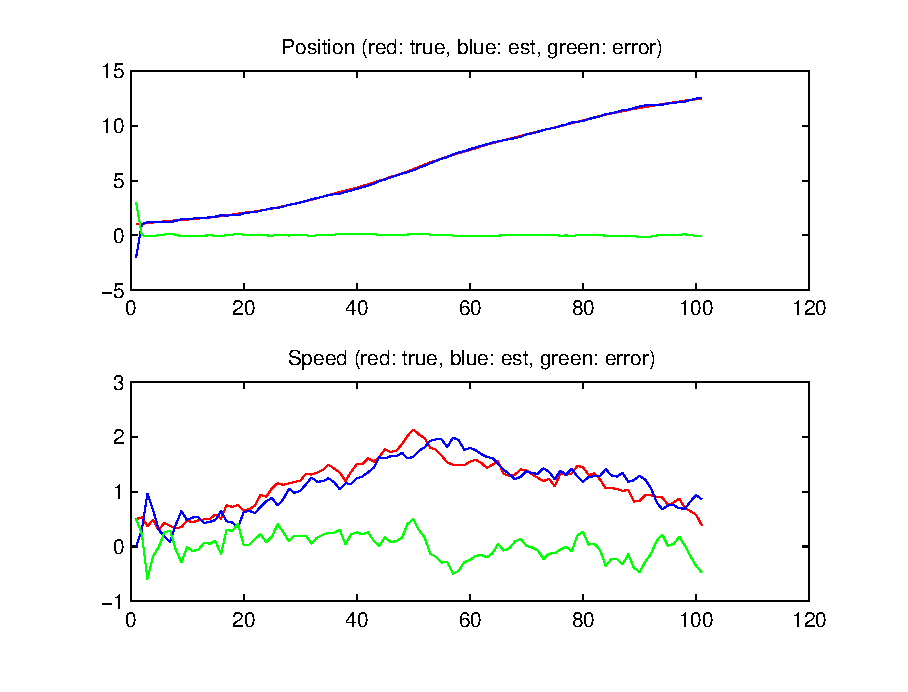
\includegraphics[width=.43\textwidth]{figures/kf/norm_error}
        }
        \label{fig:def}
      }\\
      \subfloat[High process noise: $Q\times100, R$]{
        \centerline
        {
          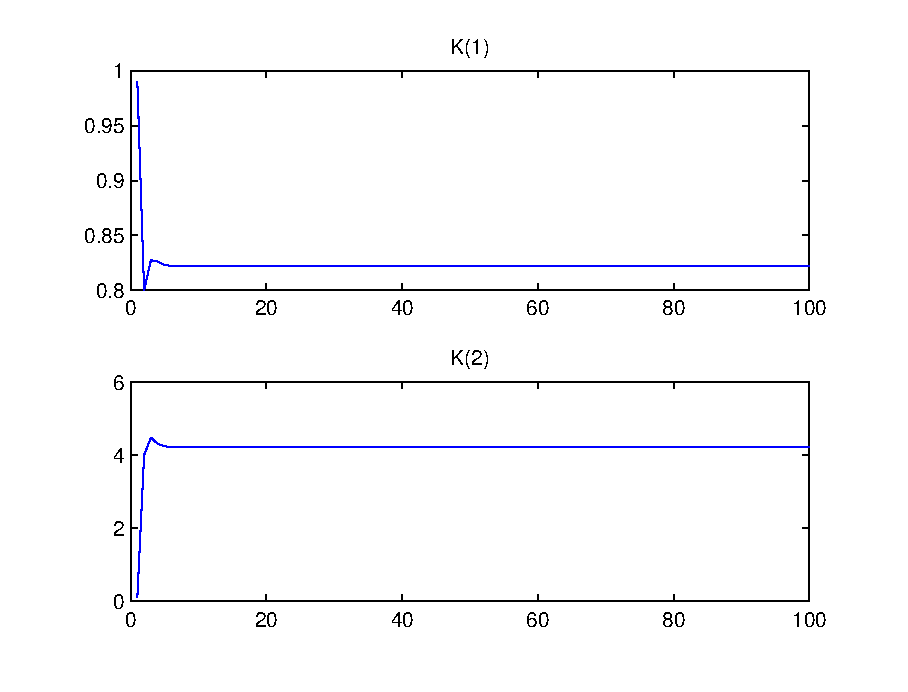
\includegraphics[width=.43\textwidth]{figures/kf/highq_kalman}
          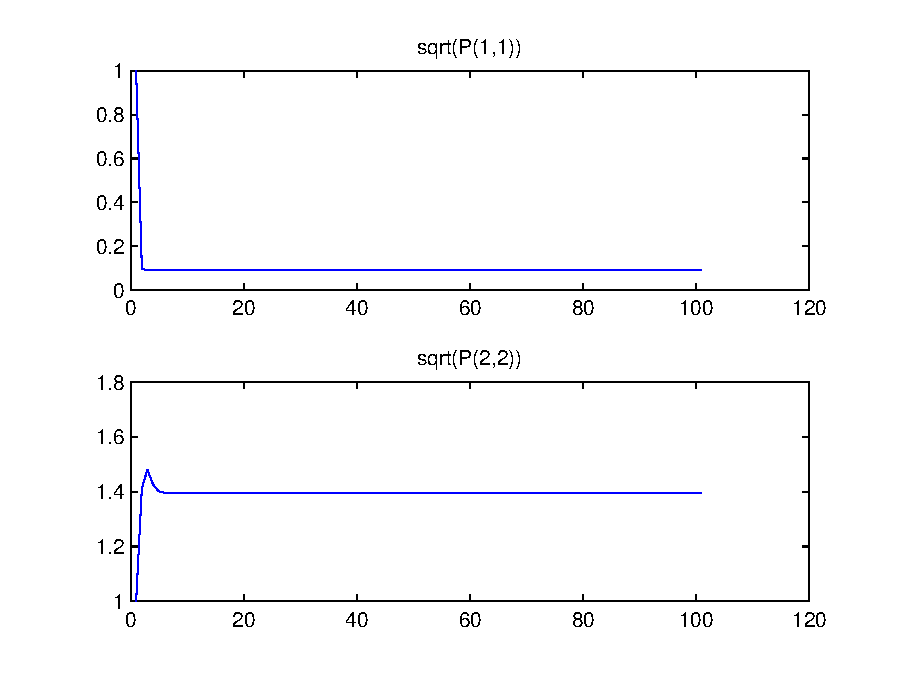
\includegraphics[width=.43\textwidth]{figures/kf/highq_covar}
          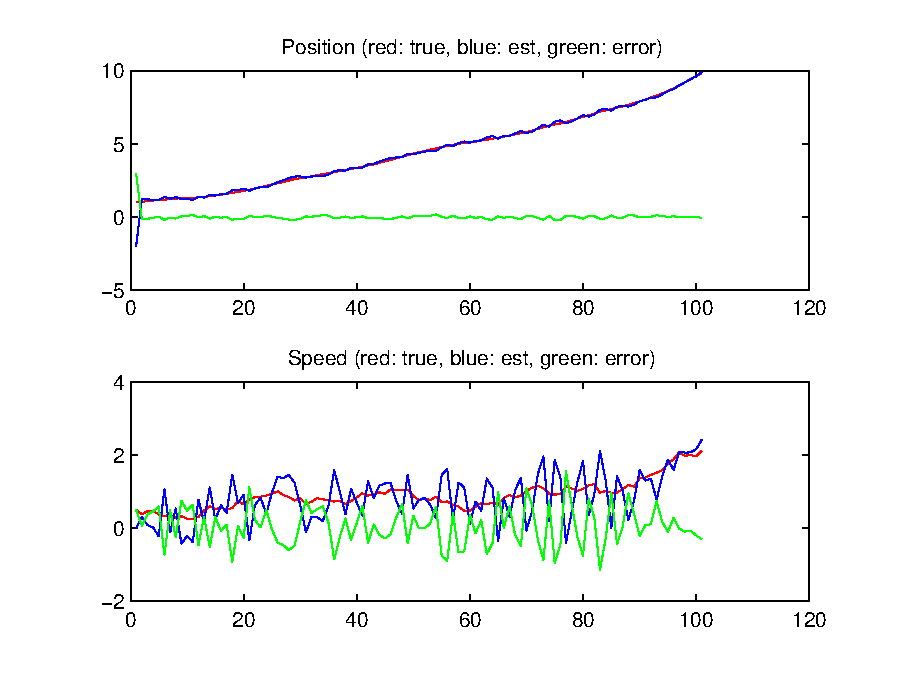
\includegraphics[width=.43\textwidth]{figures/kf/highq_error}
        }
        \label{fig:hiq}
      }\\
      \subfloat[Low process noise: $Q/100, R$]{
        \centerline
        {
          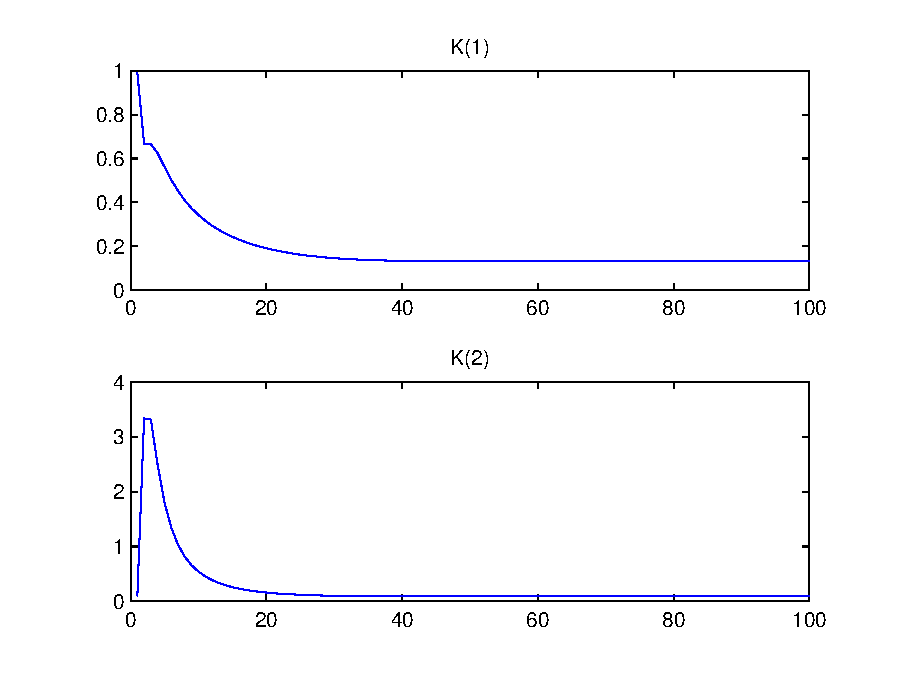
\includegraphics[width=.43\textwidth]{figures/kf/lowq_kalman}
          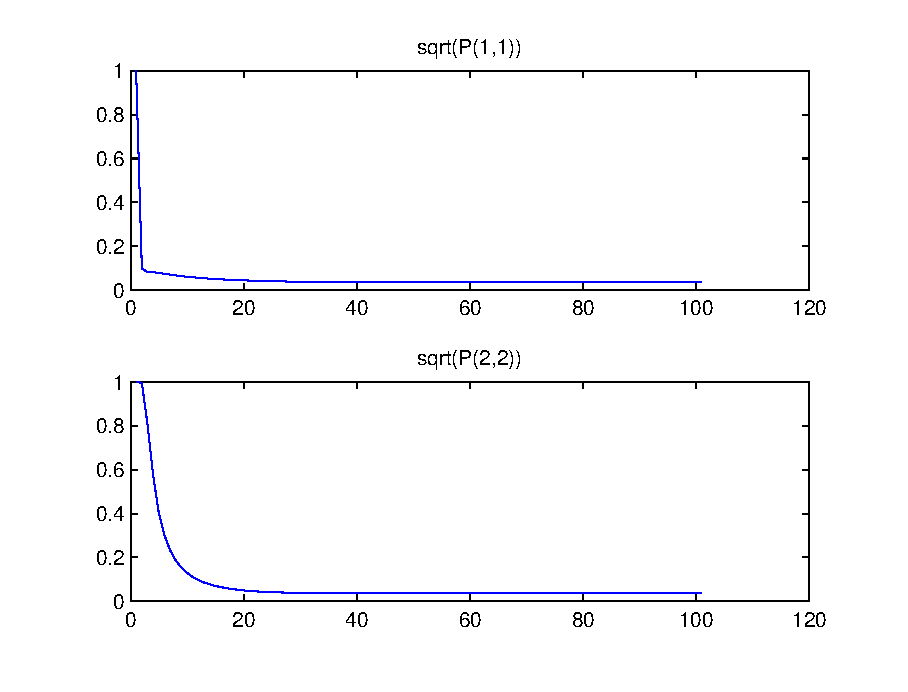
\includegraphics[width=.43\textwidth]{figures/kf/lowq_covar}
          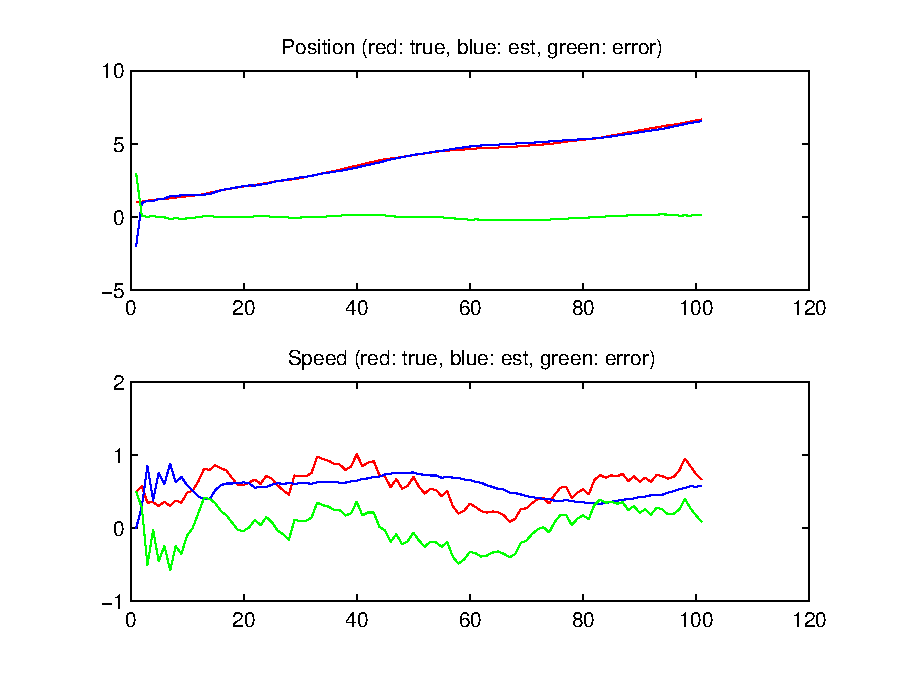
\includegraphics[width=.43\textwidth]{figures/kf/lowq_error}
        }
        \label{fig:loq}
      }\\
      \subfloat[High measurement noise: $Q, R\times100$]{
        \centerline
        {
          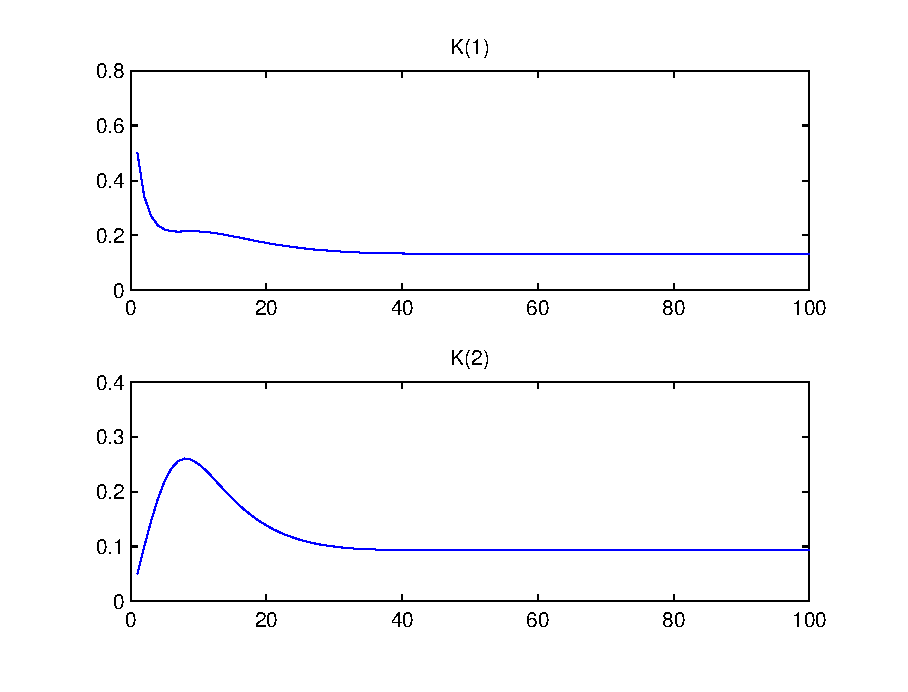
\includegraphics[width=.43\textwidth]{figures/kf/highr_kalman}
          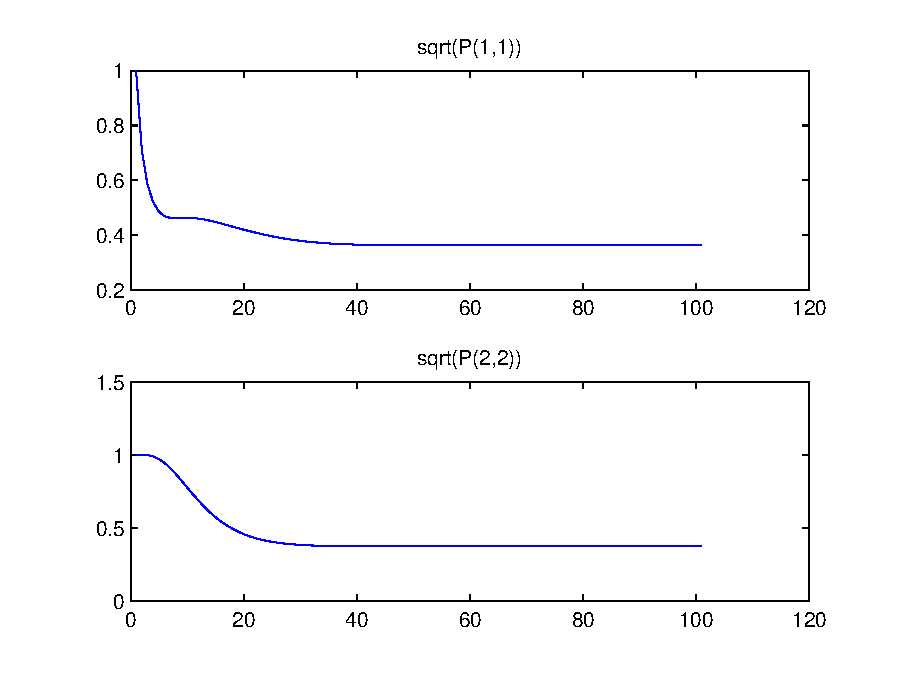
\includegraphics[width=.43\textwidth]{figures/kf/highr_covar}
          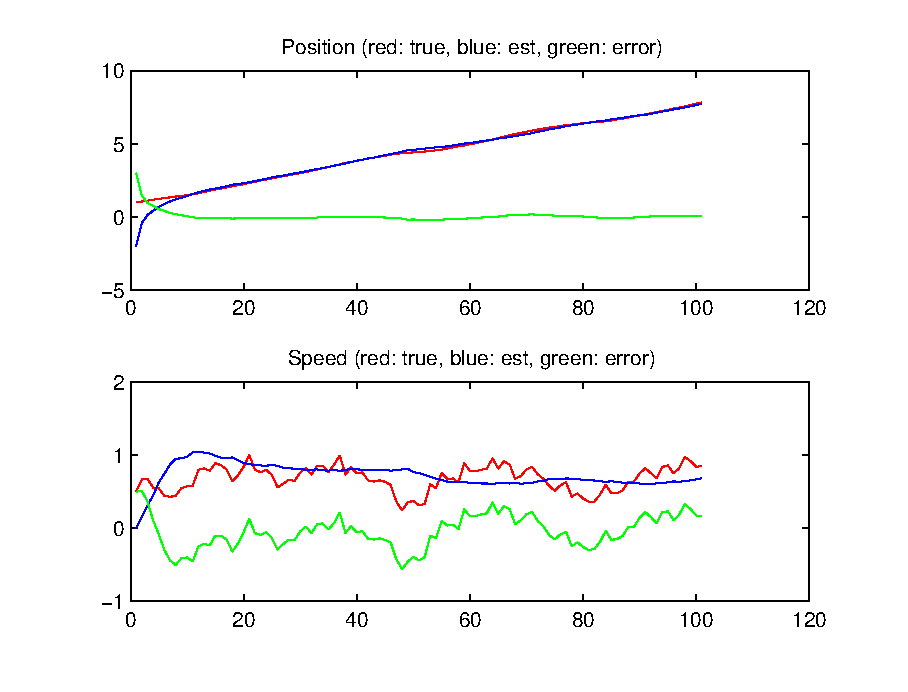
\includegraphics[width=.43\textwidth]{figures/kf/highr_error}
        }
        \label{fig:hir}
      }
      \caption{Graphs for different process and measurement noise models, from
        left to right the Kalman gain, covariance and error. By default,
        $Q=$\texttt{diag}$(0.0001,0.01)$, $R=0.01$.}
  \end{figure}
  \begin{figure}
    \renewcommand{\figurename}{Figure (cont.)}
    \ContinuedFloat
      \subfloat[Low measurement noise: $Q,R/100$]{
        \centerline
        {
          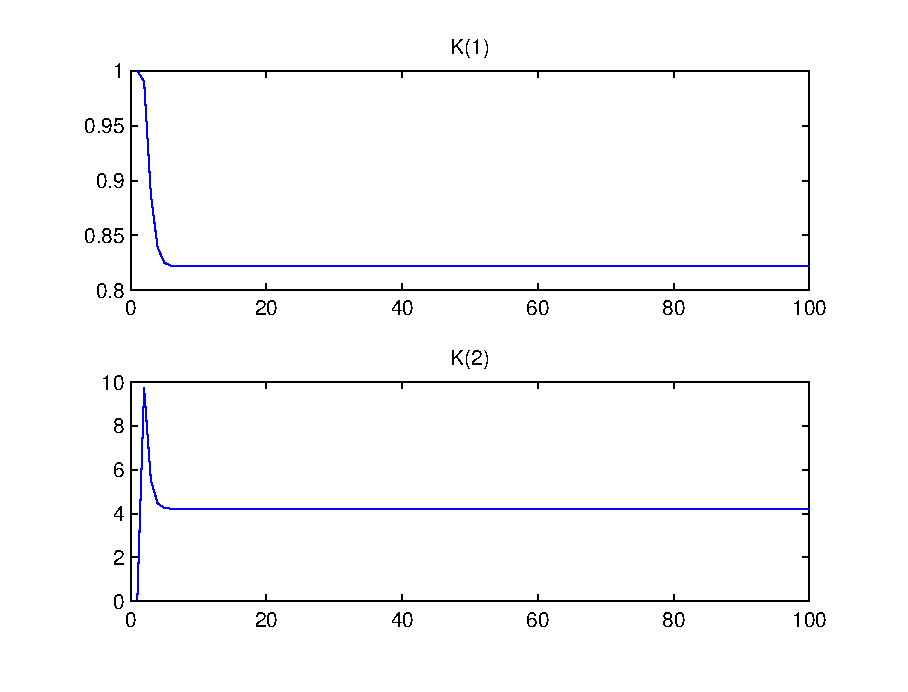
\includegraphics[width=.43\textwidth]{figures/kf/lowr_kalman}
          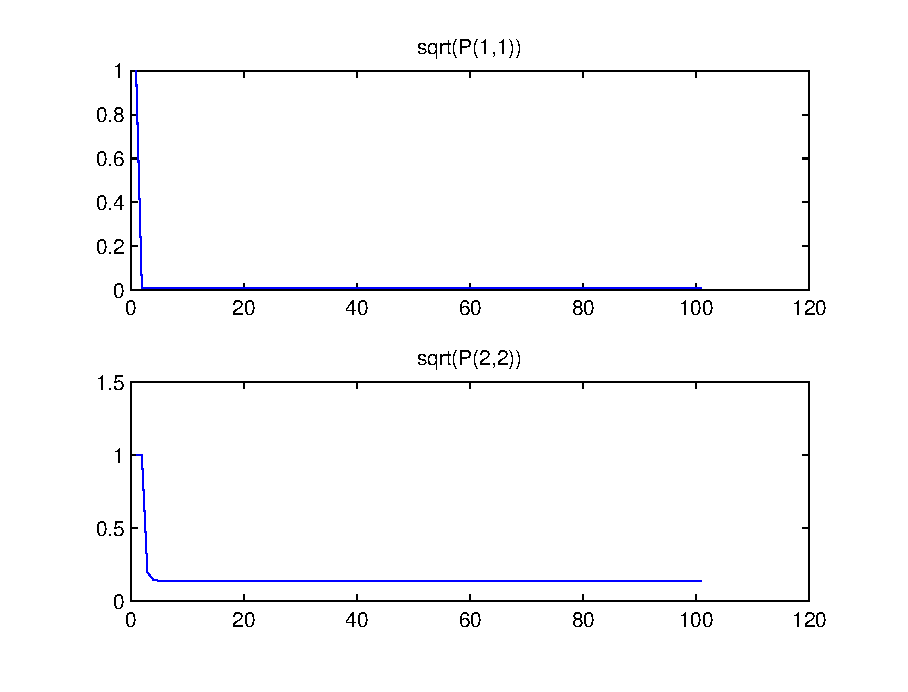
\includegraphics[width=.43\textwidth]{figures/kf/lowr_covar}
          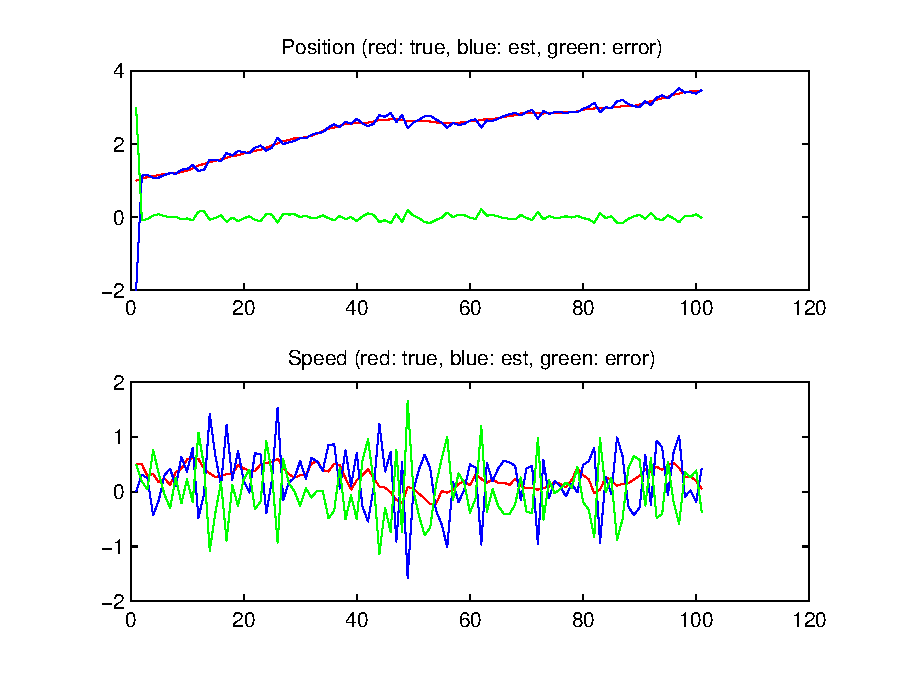
\includegraphics[width=.43\textwidth]{figures/kf/lowr_error}
        }
        \label{fig:lor}
      }
      \caption{Graphs for different process and measurement noise models, from
        left to right the Kalman gain, covariance and error. By default,
        $Q=$\texttt{diag}$(0.0001,0.01)$, $R=0.01$.}
  \end{figure}

\item Changes in the values in $P$ affect the belief state in the initial
  position. If $P$ is very high, the initial uncertainty in our estimated
  position~$\hat{x}$ is very large. When this is the case, the Kalman gain rises
  rapidly to take into account the measurements, and the systems converges in
  around the same number of time steps as with some lower values of
  $P$. Particularly noticeable is a peak in the gain for the velocity at time
  step 2, after which the gain decays quickly, indicating that the state
  uncertainty is decreasing, so it can be taken into account more. For $K>
  100$, the maximum value of the peak does not exceed 10. If $P$ is low, then
  we believe that our initial $\hat{x}$ is a very good estimate of the true
  state. This can have an effect on the convergence of the system---if the true
  state is actually far from the initial estimate of $\hat{x}$, then the state
  transition is trusted more than it should be, leading to a longer convergence
  time, due to the need to compensate for the excessive initial certainty.
\end{enumerate}
\newpage
\subsection{EKF Localisation}
\begin{enumerate}[resume]
\item The prediction step is used to generate the prior $\overline{bel}(x_t)$,
  which is our belief about the state of the robot before the measurements are
  taken into account. The update step integrates $\overline{bel}(x_t)$ and the
  probability of making the observed measurement.
  \begin{align}
    \overline{bel}(x_t)&=\int{p(x_t \mid
      u_{1:t},x_{t-1})bel(x_{t-1})dx_{t-1}}\\\eqname{Prediction step} \\
    bel(x_t)&=\eta p(z_t \mid x_t,M)\overline{bel}(x_t)\\\eqname{Update step}\\
    p(x_t\mid u_{1:t},z_{1:t},\bar{x}_0,M)&=\underbrace{\eta p(z_t \mid x_t,M)\underbrace{\int{p(x_t \mid
      u_t,x_{t-1})p(x_{t-1} \mid
      z_{1:t-1},u_{1:t-1},\bar{x}_0,M)dx_{t-1}}}_\text{Prediction
    Step}}_\text{Update step}\label{eq:q5-3}
  \end{align}
  In \eqref{eq:q5-3}, the integral is equivalent to $\overline{bel}(x_t)$, and forms
  the prediction step. Multiplying this by the normalisation constant and
  measurement probability $\eta p(z_t \mid x_t,M)$ gives the update step.
\item The assumption that measurements are independent of each other is valid,
  so long as some conditions are fulfilled. If we know that the noise is
  uncorrelated, then the measurements are unbiased, as the noise on each
  measurement is white. This means that we can expect measurements to be evenly
  distributed between values which are too small and too large. If this holds,
  then as the number of measurements tends towards infinity, we will be closer
  and closer to the true measurement value. If the sensor noise is correlated,
  then we cannot make an independence assumption. In general, the measurements
  at a single time step have a single dependency, the true state at that time
  step. However, each measurement is unaffected by the previous ones---assuming
  the sensor behaves in the same way for each measurement.
\item The value of $\delta_m$ is within the bounds $[0,1]$. The value of
  $\delta_m$ defines the confidence level in the sensor return values. A high
  value indicates high confidence in the measurements, which means that only
  values at the very ends of the tails will be rejected. A low value will result
  in more rejected associations, as there is less confidence in the
  measurements, so values closer to the centre of the distribution will also be
  rejected. If all measurements are reliable, only coming from actual features,
  then we should set $\lambda_m$ to be high, such that only measurements at the
  extreme tails will be rejected. If the measurements are unreliable, then we
  should use a lower value of $\lambda_m$ so as to ensure that only those
  measurements in which we have a high confidence are kept and integrated into
  our belief.
\item The sequential update has problems with noisy measurements, as they can
  cause inconsistencies to arise in the belief state. That is, if we receive a
  noisy measurement, and believe that it is a good measurement, we will
  integrate it into our belief, and the mean and covariance will be adjusted
  accordingly, with the mean moving towards the measurement, and the covariance
  being reduced. However, in actual fact, we have not really decreased the
  covariance, as the measurement is noisy---we have moved the mean into a
  position which could actually be \emph{less} likely than the previous
  estimate. As a result, all subsequent measurements are affected, and the mean
  jumps around, with noise having a large effect. This effect can be mitigated
  by using the batch update, which compensates for this by averaging the noise
  by doing a single update for all of the measurements.
\item In the pseudocode, we perform a computation of the expected measurement
  $\hat{z}_t^k$, the linearised measurement model~$H_t^k$, and the measurement
  uncertainty~$S_t^k$. These computations need to be done only a single time for
  each landmark $k$, but they are instead done repeatedly for each observation
  $i$. This results in $ki$ computations of these values, whereas only $k$
  computations are needed. Pre-computing these values and then performing the
  computation of $\nu_t^{i,k}$, $\nu_t^{i,k}$, and $\psi_t^{i,k}$ will result in
  a significant reduction in the computation time required, especially if there
  are a large number of observations.
\item In the batch algorithm, $\bar{\nu}_t$ and $\bar{H}_t$ have dimensions
  $2i\times 1$ and $2i\times 3$ respectively, where $i$ is the number of
  observations, compared to $2\times 1$ and $2\times 3$ for the sequential
  algorithm. This indicates that in the sequential update, each observation is
  factored into the update individually, whereas in the batch case, the
  observations are grouped together and then $K_t$, $\mu_t$ and $\Sigma_t$ are
  computed in one go with the single large matrix. As a result, the batch update
  is more expensive than the multiple sequential updates, as the matrix
  dimensions are much larger. The inversion, which has approximately
  $\mathcal{O}(n^3)$ complexity in the number of elements, becomes particularly
  costly.
\end{enumerate}
\section{Results}
Plots in this section are colour coded. Green is the ground truth, the actual
state of the robot. Red is the state of the robot estimated by the EKF. Blue is
the state of the robot based on the odometry readings.

The results of running the EKF with sequential update on the first map can be
seen in Figure~\ref{fig:map1}. We can see from the covariance graph that between
200 and 300 time steps there are two peaks in the uncertainty. This roughly
corresponds to the two corners on the right side of the map. Since this part of
the map is symmetric, the uncertainty increases as it is possible to be in
either of those two places. The overall error is very small, indicating that the
EKF performs very well in this example.

On the second map, seen in Figure~\ref{fig:map2}, we have the problem of
outliers in the measurements, coming from spurious measurements or sensor
error. While the odometry is of bad quality as always, it is very important that
we properly determine the uncertainty, as if we are overly reliant on
measurements, the filter will diverge, with large deviations from the true path
of the robot. With an 100 times larger uncertainty in the process model, the
filter diverges very quickly and gets stuck at the bottom of the ellipse. With
10 times larger uncertainty, the tracking is reasonable until the top left part,
where the filter gets stuck. When the noise model is correctly chosen, outliers
are correctly detected and the filter tracks the true state well. We see an
interesting pattern in the covariance, which corresponds to encountering each of
the landmarks. Each time we see one, the uncertainty increases, as the position
and heading are somewhat correlated with the measured position of the landmark.

The third map has no outliers, but instead has problems with high noise
measurements affecting the sequential update. Figure~\subref*{fig:m3seq} and (b)
show the runs for sequential and batch updates of the EKF respectively. Using
the sequential update, the noisy measurements result in a large deviation from
the true state. In contrast, with the batch update there is only slight
deviation from the true state. We again see a sawtooth pattern in the
covariance, corresponding to each landmark being encountered. The $x$ and $y$
covariances appear to follow a sine curve. This may be as a result of the
computation of the position from the measurements, which include sinusoids.

\begin{figure}
  \centerline
  {
    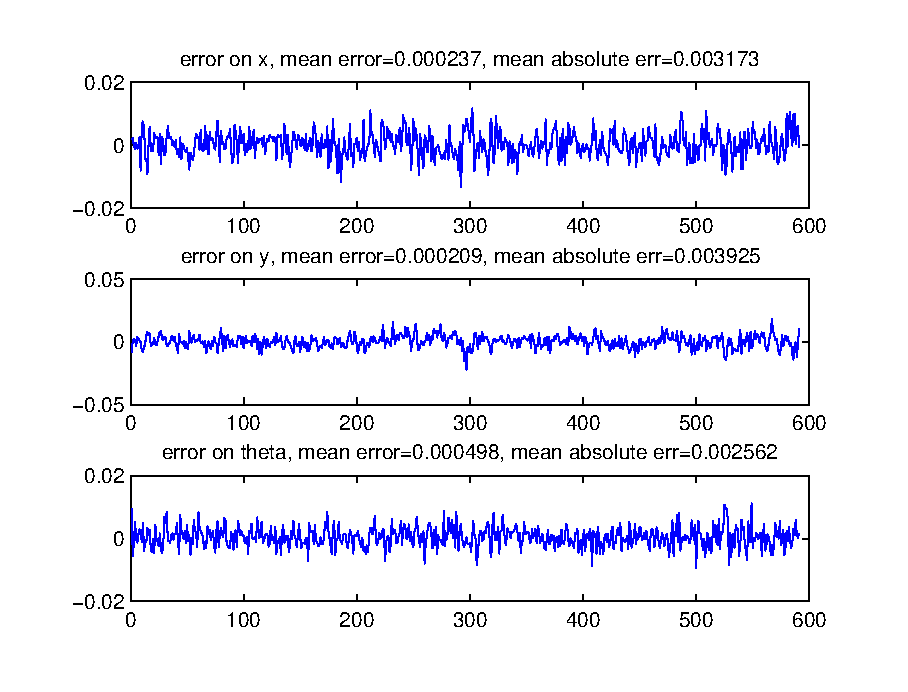
\includegraphics[width=.43\textwidth]{figures/ekf/map1_seq_error}
    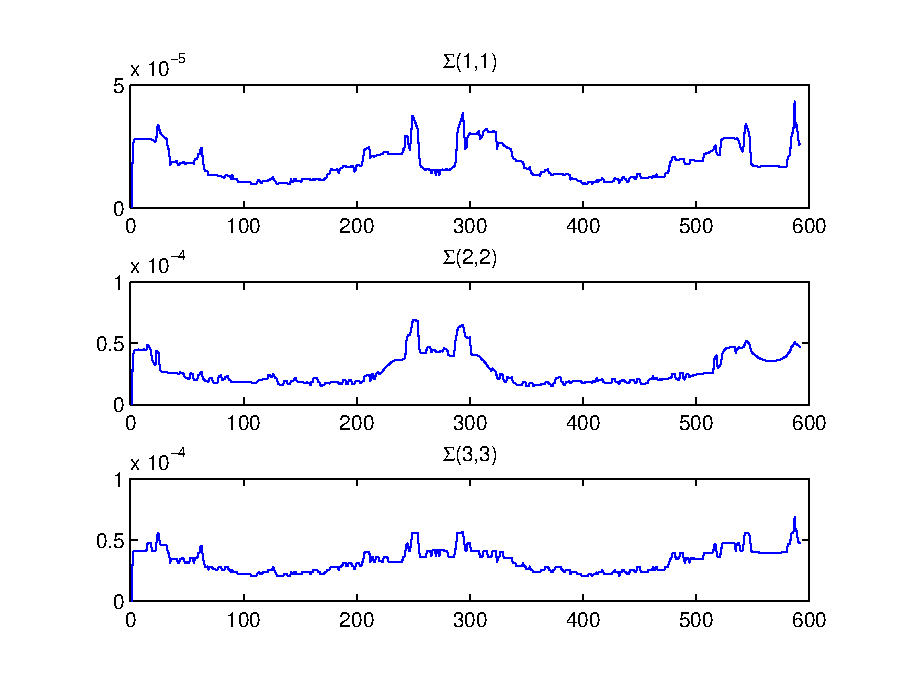
\includegraphics[width=.43\textwidth]{figures/ekf/map1_seq_sigma}
    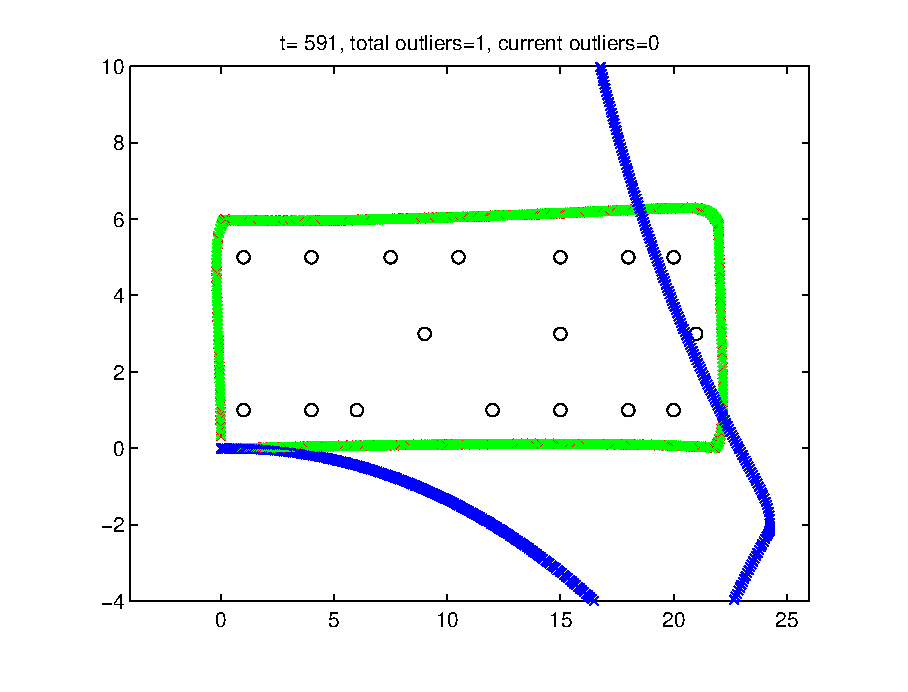
\includegraphics[width=.43\textwidth]{figures/ekf/map1_seq_motion}
  }
  \caption{A run of the EKF on the first test map. This gives an indication of
    the poor quality of odometry data. The noise models used were
    $R=$\texttt{diag}$(0.01^2, 0.01^2, 0.0175^2)$, $Q=$\texttt{diag}$(0.01^2,
    0.0175^2)$.}
  \label{fig:map1}
\end{figure}


\begin{figure}
  \centerline
  {
    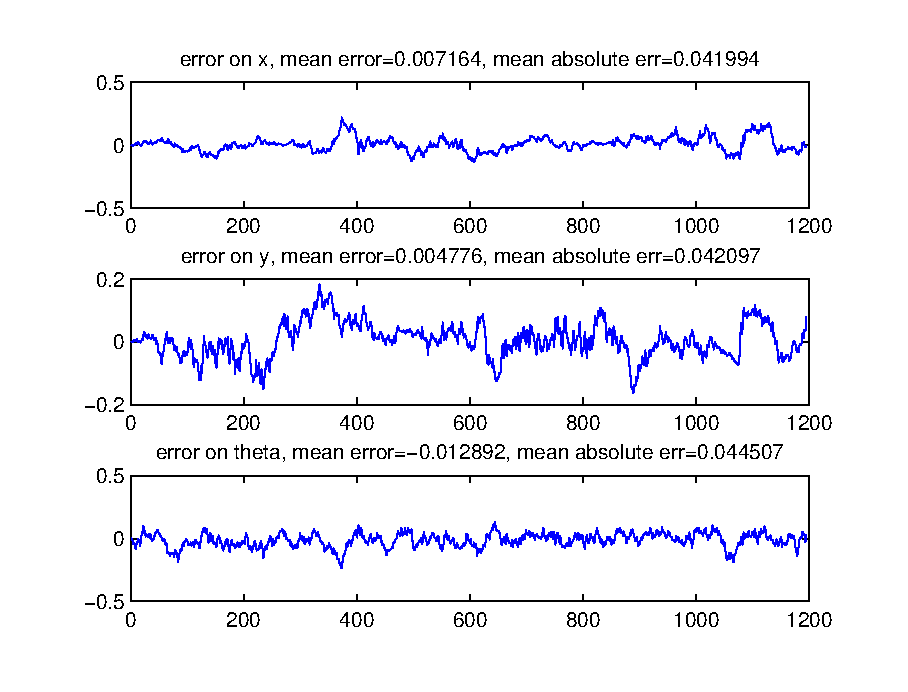
\includegraphics[width=.43\textwidth]{figures/ekf/map2_seq_error}
    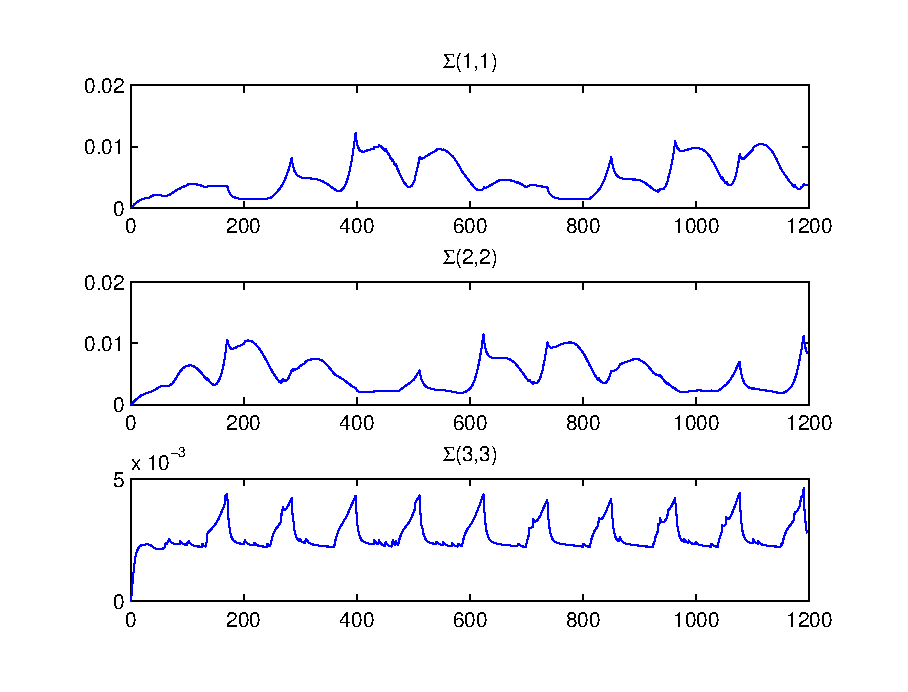
\includegraphics[width=.43\textwidth]{figures/ekf/map2_seq_sigma}
    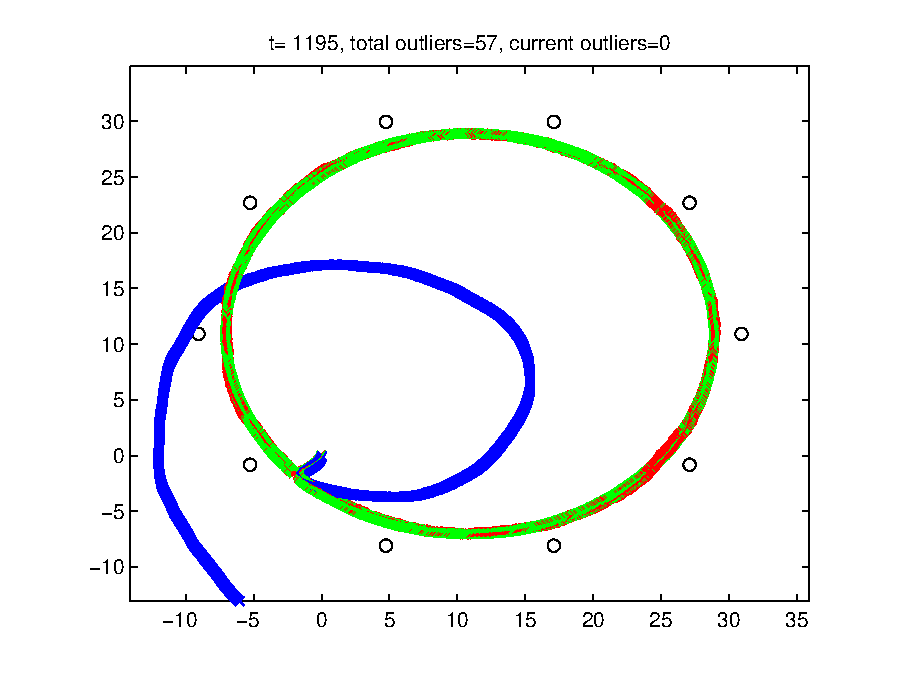
\includegraphics[width=.43\textwidth]{figures/ekf/map2_seq_motion}
  }
  \caption{Results of running the EKF on the second test map. The noise models
    used were $R=$\texttt{diag}$(0.01^2, 0.01^2, 0.0175^2)$,
    $Q=$\texttt{diag}$(0.2^2, 0.2^2)$. In this case, the noise models are
    important as outliers can cause divergence if not correctly chosen.}
  \label{fig:map2}
\end{figure}
\begin{figure}
  \subfloat[Sequential update]{
    \centerline
    {
      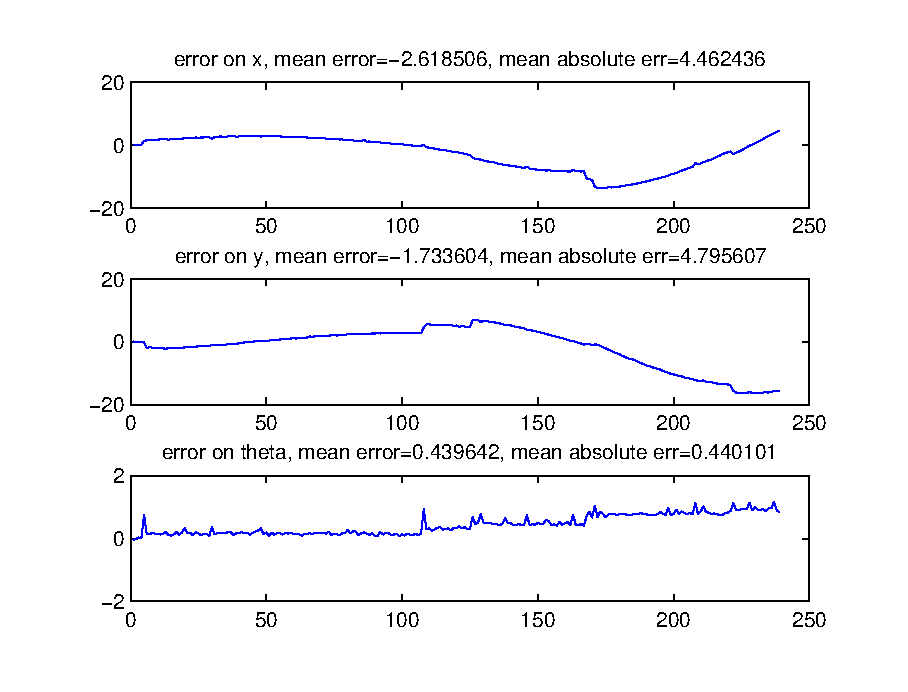
\includegraphics[width=.43\textwidth]{figures/ekf/map3_seq_error}
      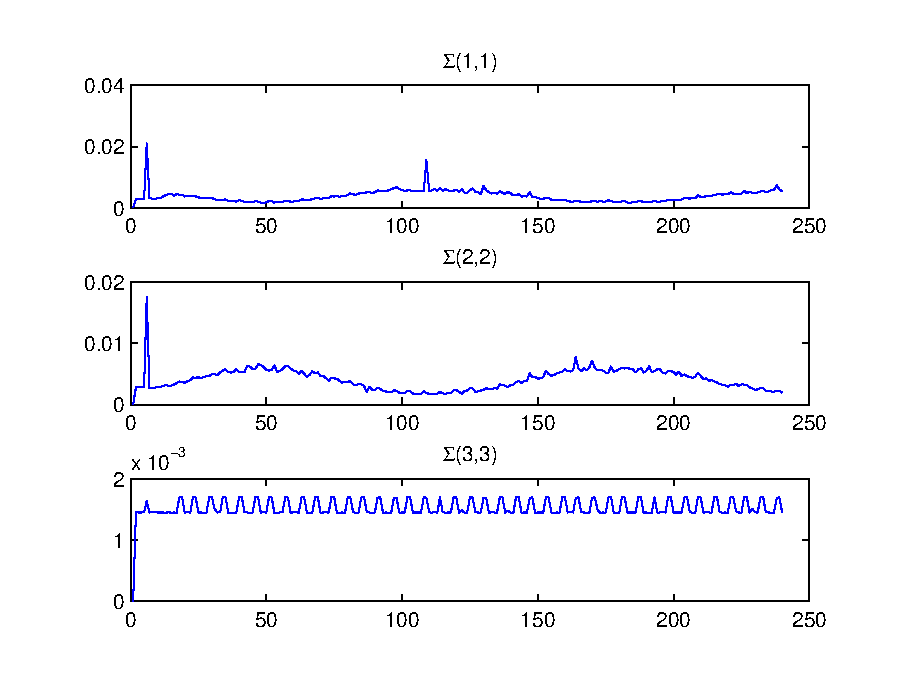
\includegraphics[width=.43\textwidth]{figures/ekf/map3_seq_sigma}
      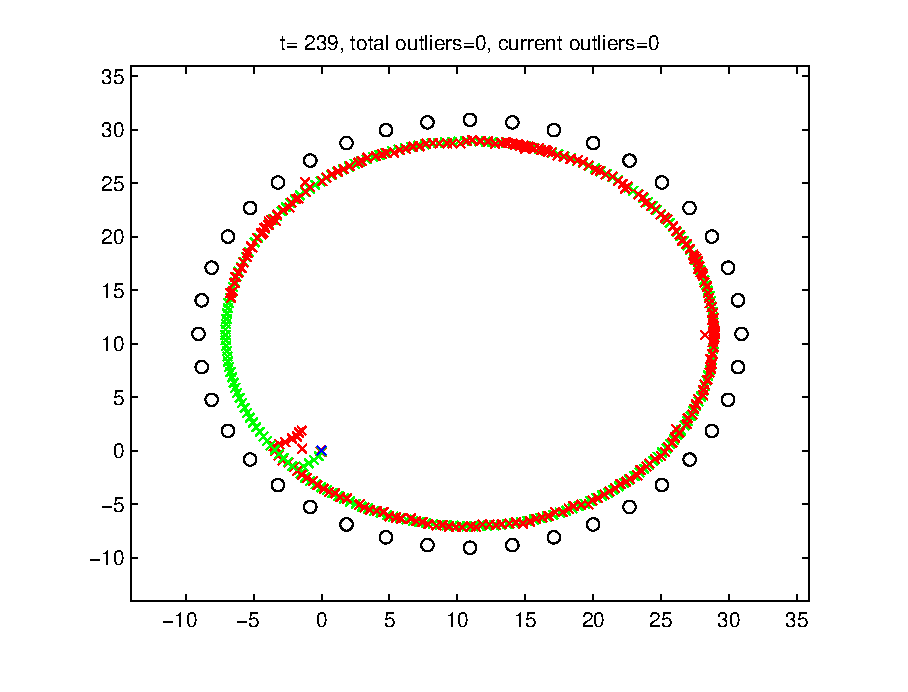
\includegraphics[width=.43\textwidth]{figures/ekf/map3_seq_motion}
    }
    \label{fig:m3seq}
  }\\
  \subfloat[Batch update]{
    \centerline
    {
      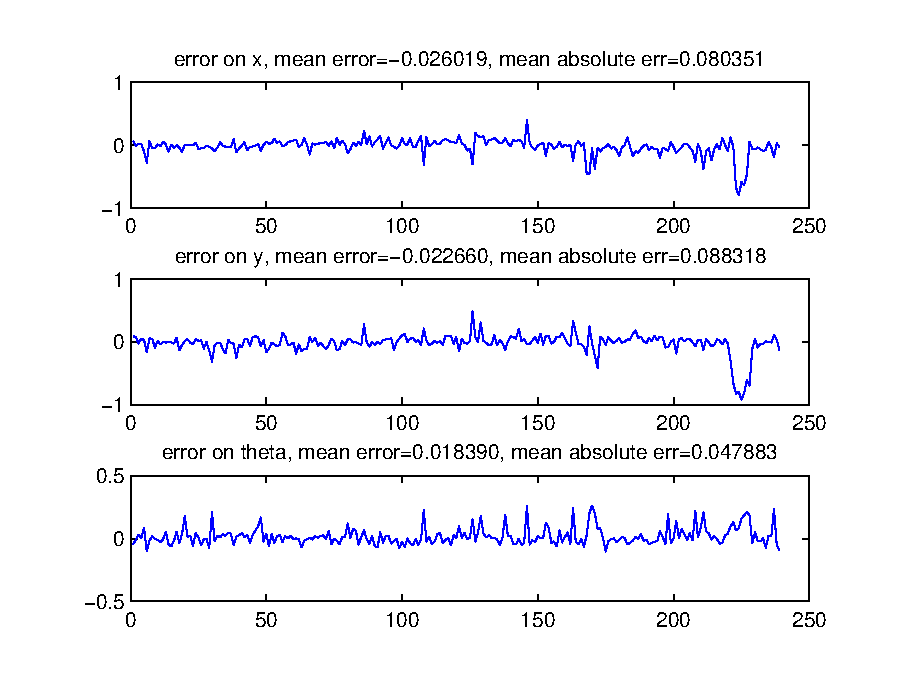
\includegraphics[width=.43\textwidth]{figures/ekf/map3_batch_error}
      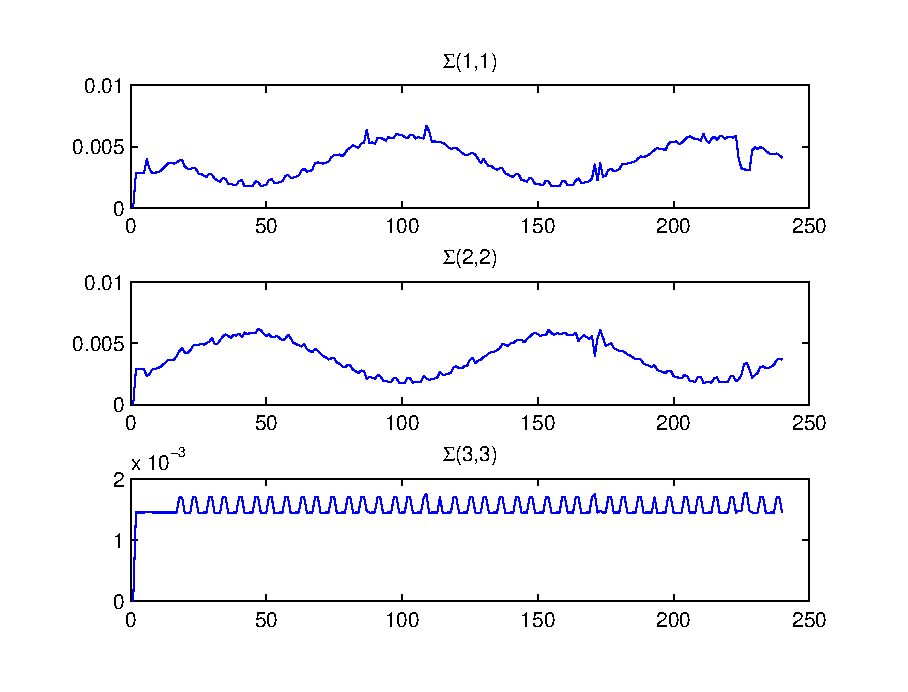
\includegraphics[width=.43\textwidth]{figures/ekf/map3_batch_sigma}
      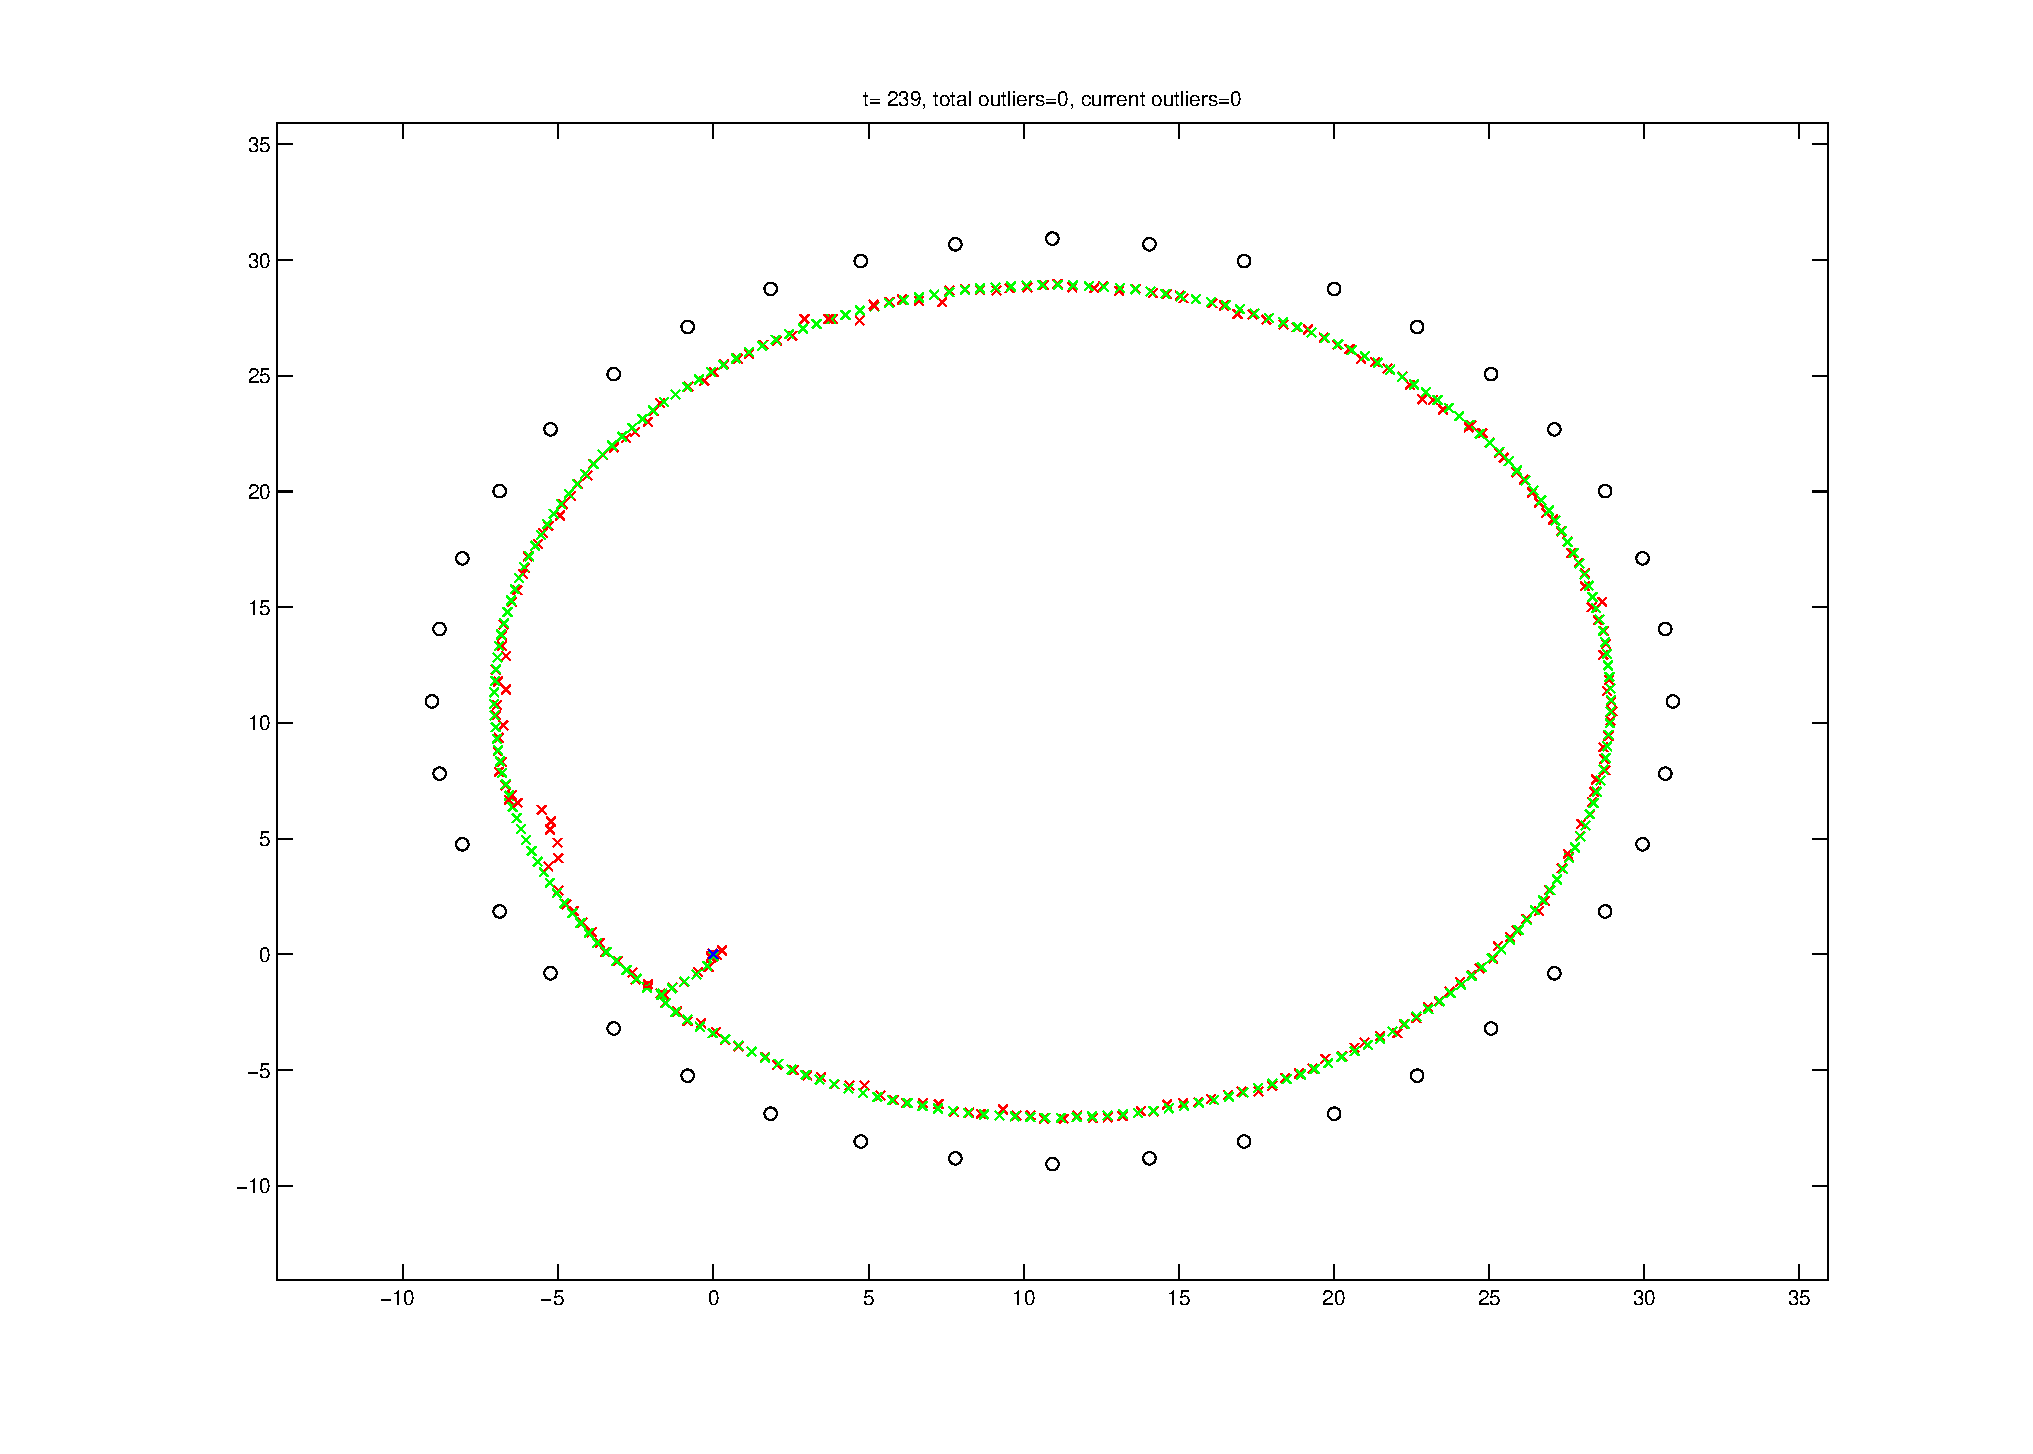
\includegraphics[width=.43\textwidth]{figures/ekf/map3_batch_motion}
    }
    \label{fig:m3batch}
  }
  
  \caption{Results of running the EKF on the third test map. The noise models
    used were $R=$\texttt{diag}$(1, 1, 1)$, $Q=$\texttt{diag}$(0.1^2,
    0.1^2)$.}
  \label{fig:map3}
\end{figure}

\end{document}
